\section{Motivating Example} 

\tmcmt{Need a better run-in to this section - TFM to write.}

\tmcmt{Rajdeep, is this this a running example for section IV only? It doesn't get referred to later. Can we discuss please?}

%
We present a motivating example. 
%  
Figure~\ref{intro-fig2} gives a Verilog RTL design (on the left) with 
two sequential blocks (modeled with always blocks) and a combinational block 
(modeled with an assign statement). It also contains an initial block that 
initializes the state-holding elements. The procedural blocks contain 
non-blocking statements, shown as \texttt{(<=)}.  Figure~\ref{intro-fig1} 
gives the synthesized hardware (on the left) for the Verilog RTL design 
of Figure~\ref{intro-fig2}, while the formal semantics of the RTL is given 
on the right side of Figure~\ref{intro-fig1}.  The adder circuit and 
multiplier circuit in the synthesized hardware are shown in vertical boxes, 
denoted by \texttt{ADDER} and \texttt{MUL}, respectively.  While the 
registers are shown as square boxes with the name of register marked 
inside the box and the two Multiplier circuits are denoted by trapezium 
shapes, with two input lines, one select line and one output line.  
The formal semantics on the right side of Figure~\ref{intro-fig1} 
contains the semantics of the combinational logic and sequential logic, 
with respect to the temporal variable $t$. 
%
The Verilog RTL is translated into software netlist in C, as shown on the 
right side of Figure~\ref{intro-fig2}.  The \texttt{main()} procedure of 
the software netlist is shown on the right side of Figure~\ref{intro-fig3}, 
which also contains the initial block.
%  
The details of the translation are explained in subsequent sections.  
We are interested in verifying the correctness of the Verilog RTL design 
against safety properties. 
%

Figure~\ref{intro-fig3} gives the safety properties that are checked 
against the RTL design of Figure~\ref{intro-fig1}.  The column on the 
left of Figure~\ref{intro-fig3} 
gives the SVA properties denoted by the property identifier 
$P0 \ldots P5$ and the column on the right gives the 
corresponding assertions in the software netlist.  The properties 
in Figure~\ref{intro-fig3} are of two types - global safety properties, 
and temporal properties containing the implication construct \texttt{(|->)} of SVA.  
The translation of SVA to assertions in the software netlist is described 
in detail in Section~\ref{prop}. 
%  
Intuitively, the \texttt{\#\#N} delay operator in SVA is modeled by invoking 
the top level procedure \texttt{top} in the software netlist $N$ times.  
Since we are interested in property verification of RTL designs by translating 
them to software netlist, so we consider the notion of equivalence between 
the Verilog RTL and the software netlist that preserves both the 
input-output behavior and the validity of all assertions of the RTL in the 
software netlist. 
%
\begin{figure}[t]
\centering
\scriptsize
\begin{tabular}{|l|l|}
\hline
 Verilog RTL & Software netlist \\
\hline
\begin{lstlisting}[mathescape=true,language=Verilog,basicstyle=\footnotesize\ttfamily]
module top(clk, a, c, out); 
input clk , a;
output [1:0] c;
output reg [3:0] out;
reg b,e; reg [1:0] d;
initial begin
  b=0;d=2'b0;
  e=0;out=4'b0;
end
assign c = e ? 1'b0 : d; 
always @(posedge clk) 
begin
 b<=a;
 if(b) e <= b; 
 else  e <= 0; 
 d <= e + 1;
end
always @(posedge clk) 
begin
  out <= d*d;
end  
endmodule
\end{lstlisting}
&
\begin{lstlisting}[mathescape=true,language=C]
struct state_elements_top {
  unsigned int b,e;
  unsigned char d,out;
};
struct state_elements_top u1;

void top(unsigned int clk, 
 unsigned int a, 
 unsigned char *c, 
 unsigned char *out) {
 // shadow variables 
 unsigned int b_old = u1.b&0x1;
 unsigned char d_old = u1.d&0x3;
 unsigned int e_old = u1.e&0x1;
  
 u1.b = a;
 if(b_old) 
  u1.e = b_old&0x1;
 else
  u1.e = 0;
 u1.d = (e_old+1)&0x3;
 // update the output 
 u1.out = 
 (d_old&0x3) * (d_old&0x3);
 *out = u1.out&0xF;
 *c = u1.e ? 0 : (u1.d&0x3);
}
\end{lstlisting}
\\
\hline
\end{tabular}
\caption{Circuit to software}
\label{intro-fig2}
\end{figure}
%
\begin{figure}[t]
\scriptsize	
\centering
\begin{tabular}{|l|l|}
\hline
  System Verilog Assertions & Assertions in Software netlist \\
\hline
\begin{lstlisting}[mathescape=true,language=Verilog]
P0: assert property (d >= e);
P1: assert property ((a == 1) 
    |-> ##1 (b == 1));
P2: assert property ((a == 1) 
    |-> ##2 (e == 1));
P3: assert property ((a == 1) 
    |-> ##3 (d == 2));
P4: assert property ((a == 0) 
    |-> ##4 (out == 1));
P5: assert property ((a == 1) 
    |-> ##4 (out == 4));
\end{lstlisting}
&
\begin{lstlisting}[mathescape=true,language=C]
int main() {
 unsigned int clk, a;
 unsigned char c, out;
 // initial block
 u1.b=0;u1.d=0;
 u1.e=0;u1.out=0;
 while(1) {
  P0:assert(u1.d>=u1.e);
  if(a==1) { 
   top(clk,a,&c,&out);
   P1: assert(u1.b==1);
   top(clk,a,&c,&out);
   P2: assert(u1.e==1);
   top(clk,a,&c,&out);
   P3: assert(u1.d==2);}
  //check output register
  if(a==1) {
   top(clk,a,&c,&out);
   P5: assert(u1.out==4);}
  else if(a==0) {
   top(clk,a,&c,&out);
   P4:assert(u1.out==1); } 
 }
}
\end{lstlisting}
\\
\hline
\end{tabular}
	\caption{Property specification in SVA (on the left) and assertions of the software netlist (on the right)}
\label{intro-fig3}
\end{figure}
%
\begin{figure}[t]
%\scriptsize  
\centering
\begin{tabular}{|l|l|}
\hline
  Synthesized Hardware & Formal Semantics \\
\hline
\begin{minipage}{3.9cm}
\centering
\vspace{1mm}
\scalebox{.5}{\import{figures/example/}{ckt.pspdftex}}
\vspace{1mm}
\end{minipage}
&
\begin{minipage}{4.1cm}
%\centering
\scalebox{.55}{\import{figures/example/}{semantics.pspdftex}}
\end{minipage}
\\
\hline
\end{tabular}
\caption{Hardware circuit and its formal semantics}
\label{intro-fig1}
\end{figure}
%


The waveform in Figure~\ref{intro-waveform} captures the input-output behavior of the RTL design. 
%The input-output behavior of the software netlist and the RTL in figure~\ref{intro-fig2} matches 
Using state-of-the-art verifiers, we prove that the result of all assertions 
in Figure~\ref{intro-fig3} are the same in the RTL and the software netlist design. 
%
For example, the properties \texttt{P2:assert(u1.d==1);} and \texttt{P3:assert(c==1);} 
hold only for the first cycle in both RTL and software netlist, but fails in the 
subsequent cycles in both the designs.  All other properties 
hold globally in both the designs, that is, these properties are $k$-inductive 
for the same value of $k$ in the RTL and the software netlist design.
%
\begin{figure} 
\begin{center}
  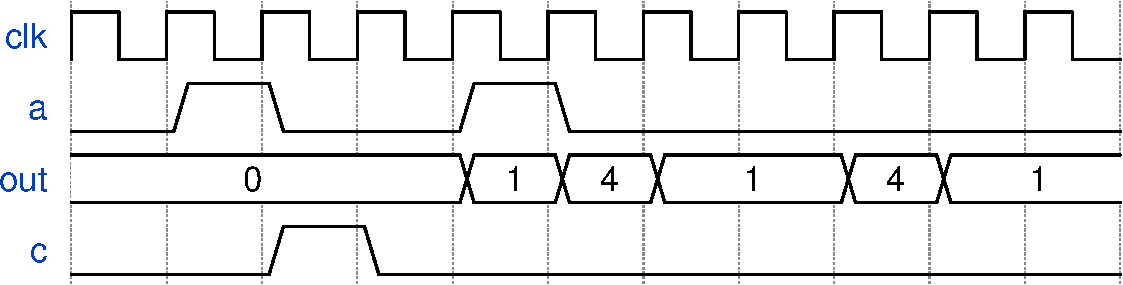
\includegraphics[width=\columnwidth]{figures/example/waveform1.pdf}%
	\caption{Waveform showing the Input-Output behavior of RTL in Figure~\ref{intro-fig2}}
\label{intro-waveform}
\end{center}
\end{figure}
%
